In this chapter, the \textit{SLDC} framework is applied the problem presented in Chapter \ref{chap:context} : the nodule malignancy assessment. This problem is effectively an instance of the objects detection and classification problem. Indeed, the goal is to diagnose malignancy by the presence or absence of cells or groups of cells having particular characteristics in digitized microscope whole-slide. This problem is a good use case for the \textit{SLDC} framework: the images are large (i.e. typically 15 giga-pixels), two distinct categories of objects must be found (namely cells and groups of cells) and some of these objects can be included into others which can be handled using dispatching and chaining.  

An introduction to the thyroid problem as well as the underlying implementation challenges are presented in Section \ref{sec:thyroid_impl_issue}. Then, the workflow developed in \cite{adeblire2013} is briefly presented and its performances are assessed in Section \ref{sec:thyroid_adeblire_algo}. Especially, some flawed steps are highlighted and some improvements are proposed. Then, the implementation of the improved workfow is detailed in section \ref{sec:thyroid_implementation}. Finally, the performances of this implementation are analyzed in Section \ref{sec:thyroid_perf}.

\section{Problem and underlying challenges}
\label{sec:thyroid_impl_issue}
The problem consists in finding cells with inclusions and proliferative architectural patterns in large digitized microscope slides. To perform this detection, a dataset containing approximately 5700 annotations was created by experts on the Cytomine platform. The major challenges involved with this problem are detailed hereafter. 

\paragraph{Image quality} While the images resolution is more than acceptable, the images themselves are by nature not very well suited for object extraction. Indeed, the objects of interests are surrounded with a lot of other undesirable objects. Moreover, due to the imprecise nature of the staining performed before digitization, some staining variations appears from one slide to another but also within a single slide. 

\paragraph{Image size} As explained in Section \ref{sssec:detection_thyroid_dataset}, the size of the images ranges from 4 giga-pixels to 18 giga-pixels. Therefore, the various processing steps should be as efficient as possible to avoid huge execution times. Also, accessing the images must be done through HTTP requests. Therefore, a particular attention should be paid to the number of requests to be executed for fetching the image. Especially, some caching policy might be needed to reduce the network time overhead. 

\paragraph{Class imbalance} The dataset of annotations is relatively balanced if all terms are considered separately. However, grouping terms for expressing the detection as a binary (or ternary) problem results in a major class imbalance, especially for the cells with inclusion versus normal cells problem. 

\paragraph{Human annotations} The human annotations are imperfect as experts usually annotate objects roughly (i.e. an annotation can be larger than the actual object). Moreover, some annotation drawing tools provided on the Cytomine platform generate particular shapes such as circles or rectangles. Assuming that an algorithm will annotate the cells more precisely, the resulting  differences in terms of geometry and information content of the crops might lead to poor results if the experts annotations are used as learning data. 


\section{First workflow}
\label{sec:thyroid_adeblire_algo}

The workflow developed by Antoine Deblire in \cite{adeblire2013} is summarized in Figure \ref{fig:workflow_adeblire}. The idea behind this workflow is fairly simple. A first segmentation is applied to extract standalone cells and architectural patterns (step 4.3). The detected objects are then differentiated using their area and circularity (step 4.4) and dispatched to a classifier (steps 4.6). Especially, architectural patterns are classified as proliferative or non-proliferative by a first classifier and the cells are classified as inclusion or normal by a second one. Then, architectural patterns are segmented again (step 4.5) to extract the cells they contain and those cells are also passed to the cell classifier. 

\begin{figure}
	\center
 	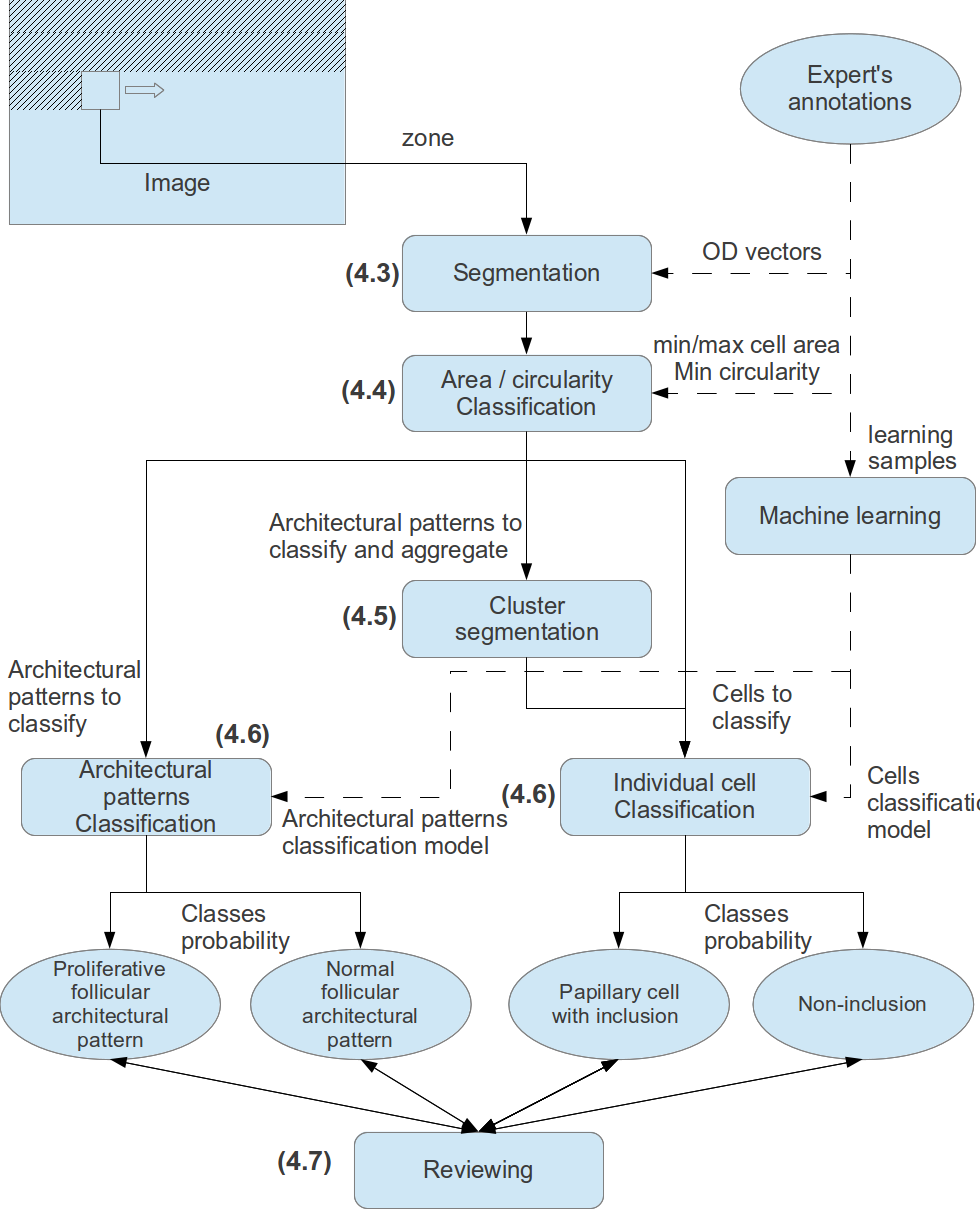
\includegraphics[scale=0.95]{image/adeblire_workflow.png}
	\caption{Antoine Deblire's workflow (source: \cite{adeblire2013})}
	\label{fig:workflow_adeblire}
\end{figure}

\subsection{Segmentation procedures}
The first segmentation procedure was designed for processing the whole slide and relies on a process called color deconvolution \cite{ruifrok2001quantification}. This process consists in retrieving the tissues stains concentration from the RGB image. It appears that cells and patterns have a high concentration of a certain stain in the project images. Therefore, a first segmentation mask is generated by thresholding an image of which each pixel contains an integer value representing the stain concentration for the same pixel in the original image. Some morphological operations are then applied in order to remove noise and fill unwanted holes. Some example segmentations are provided in Figure \ref{fig:first_seg_examples}. It seems that the procedure is able to detect most of the objects of interest although it sometimes fails at covering the whole object area. For instance in the third example image, there is a hole in the mask inside the pattern and this hole covers some cells that should be included in the mask. On the fourth example, one can see three standalone objects above the central pattern. Those objects' masks are smaller than their corresponding cells.

\begin{figure}
	\center
%	\subfigure{
%		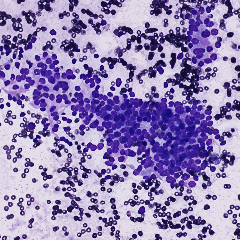
\includegraphics[scale=0.5]{image/slide_segmentation_0_in.png}
%		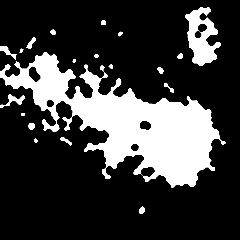
\includegraphics[scale=0.5]{image/slide_segmentation_0_out.png}
%		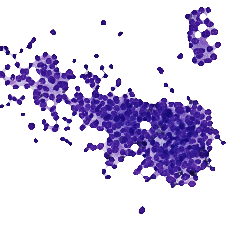
\includegraphics[scale=0.5]{image/slide_segmentation_0_masked.png}
%	} \\
%	\subfigure{
%		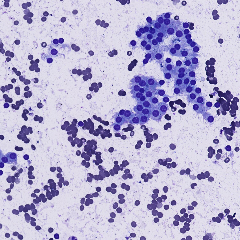
\includegraphics[scale=0.5]{image/slide_segmentation_1_in.png}
%		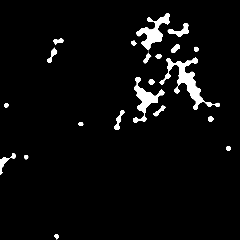
\includegraphics[scale=0.5]{image/slide_segmentation_1_out.png}
%		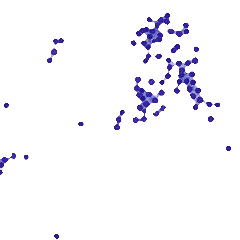
\includegraphics[scale=0.5]{image/slide_segmentation_1_masked.png}
%	} \\
%	\subfigure{
%		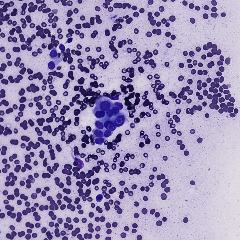
\includegraphics[scale=0.5]{image/slide_segmentation_2_in.png}
%		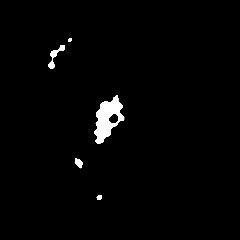
\includegraphics[scale=0.5]{image/slide_segmentation_2_out.png}
%		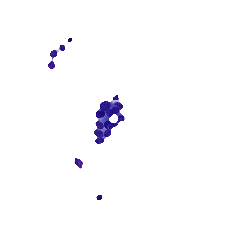
\includegraphics[scale=0.5]{image/slide_segmentation_2_masked.png}
%	} \\
%	\subfigure{
%		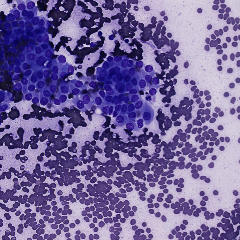
\includegraphics[scale=0.5]{image/slide_segmentation_3_in.png}
%		
\includegraphics[scale=0.5]{image/slide_segmentation_3_out.png}
%		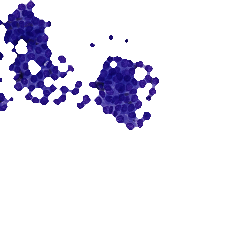
\includegraphics[scale=0.5]{image/slide_segmentation_3_masked.png}
%	}
	\caption{First segmentation - examples}
	\label{fig:first_seg_examples}
\end{figure}

The second segmentation procedure is applied to the architectural patterns and was designed to isolate individual cells inside those patterns. The implementation is a little more complicated than the first. Similarly, it starts with a color deconvolution to highlight the cells. However, the stain concentration image is not transformed into a binary mask using a fixed threshold but using Otsu's method. Using the \texttt{findContour} procedure of the OpenCV library as well as morphological operations, independent cells are located and cleaned one after the other. Finally, a watershed algorithm is applied to separate cells that intersects. Some example segmentations are provided in Figure \ref{fig:first_seg_examples}. The segmentation seems to work relatively well on "clean" patterns, that is where cells doesn't overlap much and are clearly distinguishable from the pattern background (see the first two examples in Figure \ref{fig:first_seg_examples}). One "dirty" patterns however, the segmentation performs poorly as it either returns large patches which doesn't correspond to cells or fails to separate overlapping cells.  

\begin{figure}
	\center
%	\subfigure{
%		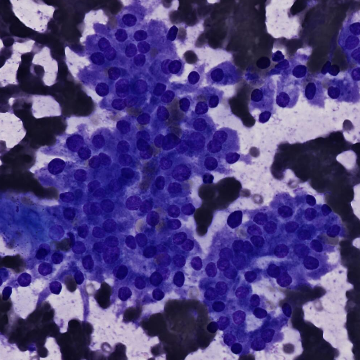
\includegraphics[scale=0.33]{image/aggr_segment_12_in.png}
%		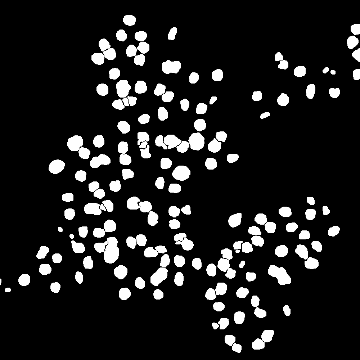
\includegraphics[scale=0.33]{image/aggr_segment_12_out.png}
%		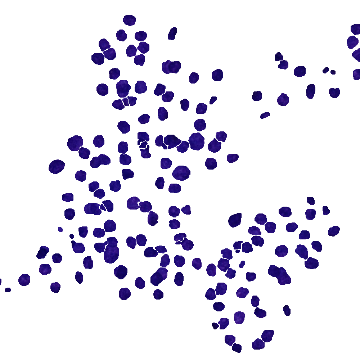
\includegraphics[scale=0.33]{image/aggr_segment_12_masked.png}
%	} \\
%	\subfigure{
%		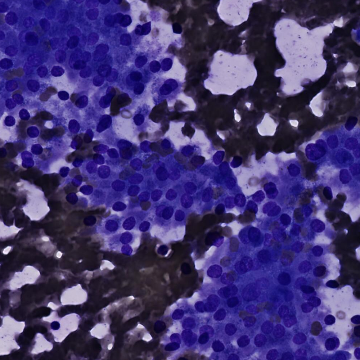
\includegraphics[scale=0.33]{image/aggr_segment_2_in.png}
%		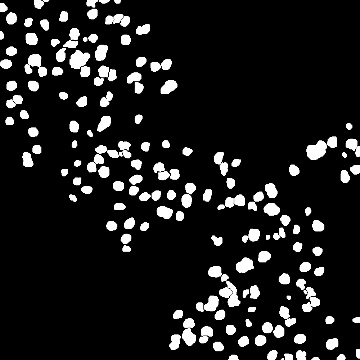
\includegraphics[scale=0.33]{image/aggr_segment_2_out.png}
%		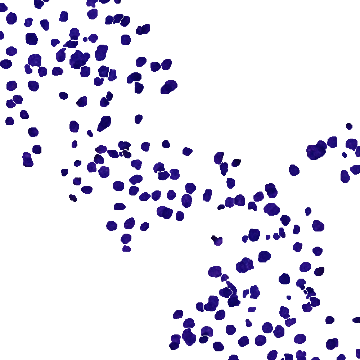
\includegraphics[scale=0.33]{image/aggr_segment_2_masked.png}
%	} \\
%	\subfigure{
%		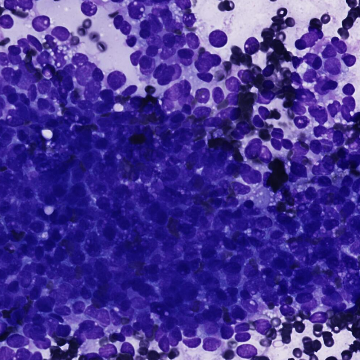
\includegraphics[scale=0.33]{image/aggr_segment_5_in.png}
%		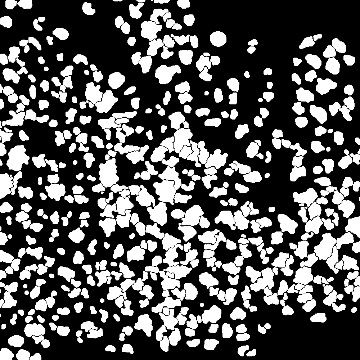
\includegraphics[scale=0.33]{image/aggr_segment_5_out.png}
%		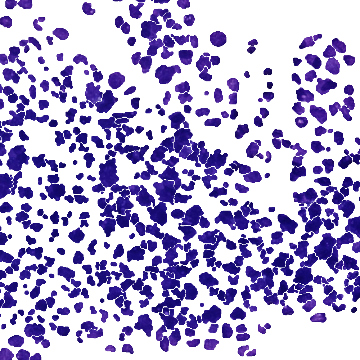
\includegraphics[scale=0.33]{image/aggr_segment_5_masked.png}
%	} \\
%	\subfigure{
%		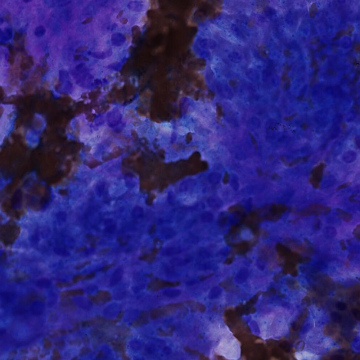
\includegraphics[scale=0.33]{image/aggr_segment_7_in.png}
%		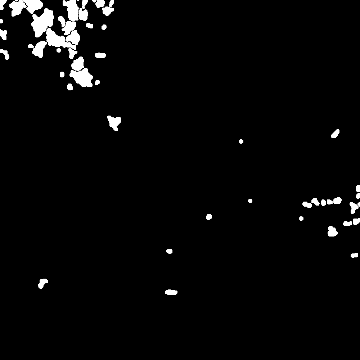
\includegraphics[scale=0.33]{image/aggr_segment_7_out.png}
%		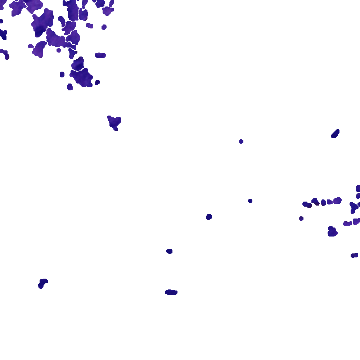
\includegraphics[scale=0.33]{image/aggr_segment_7_masked.png}
%	}
	\caption{Second segmentation - examples}
	\label{fig:second_seg_examples}
\end{figure}

While the presented segmentation procedures exhibit some flaws, they were considered acceptable to test the \textit{SLDC} framework.

\subsection{Dispatching procedure}

The step (4.4) consists in dispatching detected objects into four categories: artefacts, cells, clusters and patterns. The categories \textit{artefact} and \textit{cluster} respectively correspond to irrelevant objects and to groups of cells that contains too few of them to be patterns. Even if the author distinguishes patterns and clusters at the dispatching step, objects of both categories are treated equally in the subsequent steps of the algorithm. That is, they are first evaluated by the pattern classifier (for assessing whether they are proliferative or not) and they then are re-segmented. The dispatching is based on four parameters, the cell minimum and maximum areas (respectively, $A_{min}$ and $A_{max}$), the cell minimum circularity $C_{min}$ and the minimum number of cells per pattern $N_{min}$. The values of those parameters are given in Table \ref{tab:adeb_disp_rules}. 

Given $A$ the area of the object of interest, the dispatching rules can be summarized as follows:

\begin{itemize}
	\item \textbf{Artifact}: every object having an area less than $A_{min}$ or and area less than $A_{max}$ and a circularity less then $C_{min}$
	\item \textbf{Cell}: every object having an area such that $A_{min} < A < A_{max}$ and a circularity greater than $C_{min}$
	\item \textbf{Clusters}: every object of which the area is greater than $A_{max}$ and such that it contains at most $N_{min}$ cells:
	\[
		A_{max} < A < N_{min} \times A_{max}
	\]
	\item \textbf{Patterns}: all objects which don't match one of the rule above are considered patterns
\end{itemize}

\begin{table}
	\center
	\begin{tabular}{|c|c|}
		\hline
		$A_{min}$ & 31 $\mu m^2$\\
		\hline
		$A_{max}$ & 102 $\mu m^2$\\
		\hline
		$C_{min}$ & 0.7 \\
		\hline
		$N_{min}$ & 4\\
		\hline
	\end{tabular}
	\caption{Dispatching parameters presented in \cite{adeblire2013}}
	\label{tab:adeb_disp_rules}
\end{table}

The author fixed the dispatching parameters values based on the areas and circularities of experts' annotations. As explained in Section \ref{sec:thyroid_impl_issue}, using those annotations to perform such a task might not be an good idea. Especially, the computed minimum and maximum areas might be a greater than the actual minimum and maximum areas of cells. 

In order the assess whether the dispatching rules are effective for distinguishing cells from patterns, the expert annotations present on Cytomine were used. While those annotations shouldn't be used for setting the parameters, their usage for assessing the method is acceptable. Indeed, in this case, only a qualitative analysis is performed. 

The histograms given in Figures \ref{fig:hist_area_cell_vs_pattern} and \ref{fig:hist_circ_cell_vs_pattern} respectively show the area and circularity distributions of the experts' annotations. First, it appears that, whatever the metric, there is a substantial overlapping between the cells' and patterns' distributions. This has a major consequence for the dispatching procedure presented above. Indeed, as it relies on simple thresholdings, it is ineffective at separating the objects because of the overlapping. Another observation is that the parameters given in Table \ref{tab:adeb_disp_rules} are not relevant as most of the cells would be dispatched as patterns with such values. This observation is confirmed with the scatter plot shown in Figure \ref{fig:scatter_area_circ_cell_vs_pattern}. In this plot, only few cells are effectively dispatched as such (see the blue box in the top left corner of the plot), the others being dispatched as patterns. Given those observations, it is clear that the dispatching procedure must be re-worked.

\begin{figure}
	\center
 	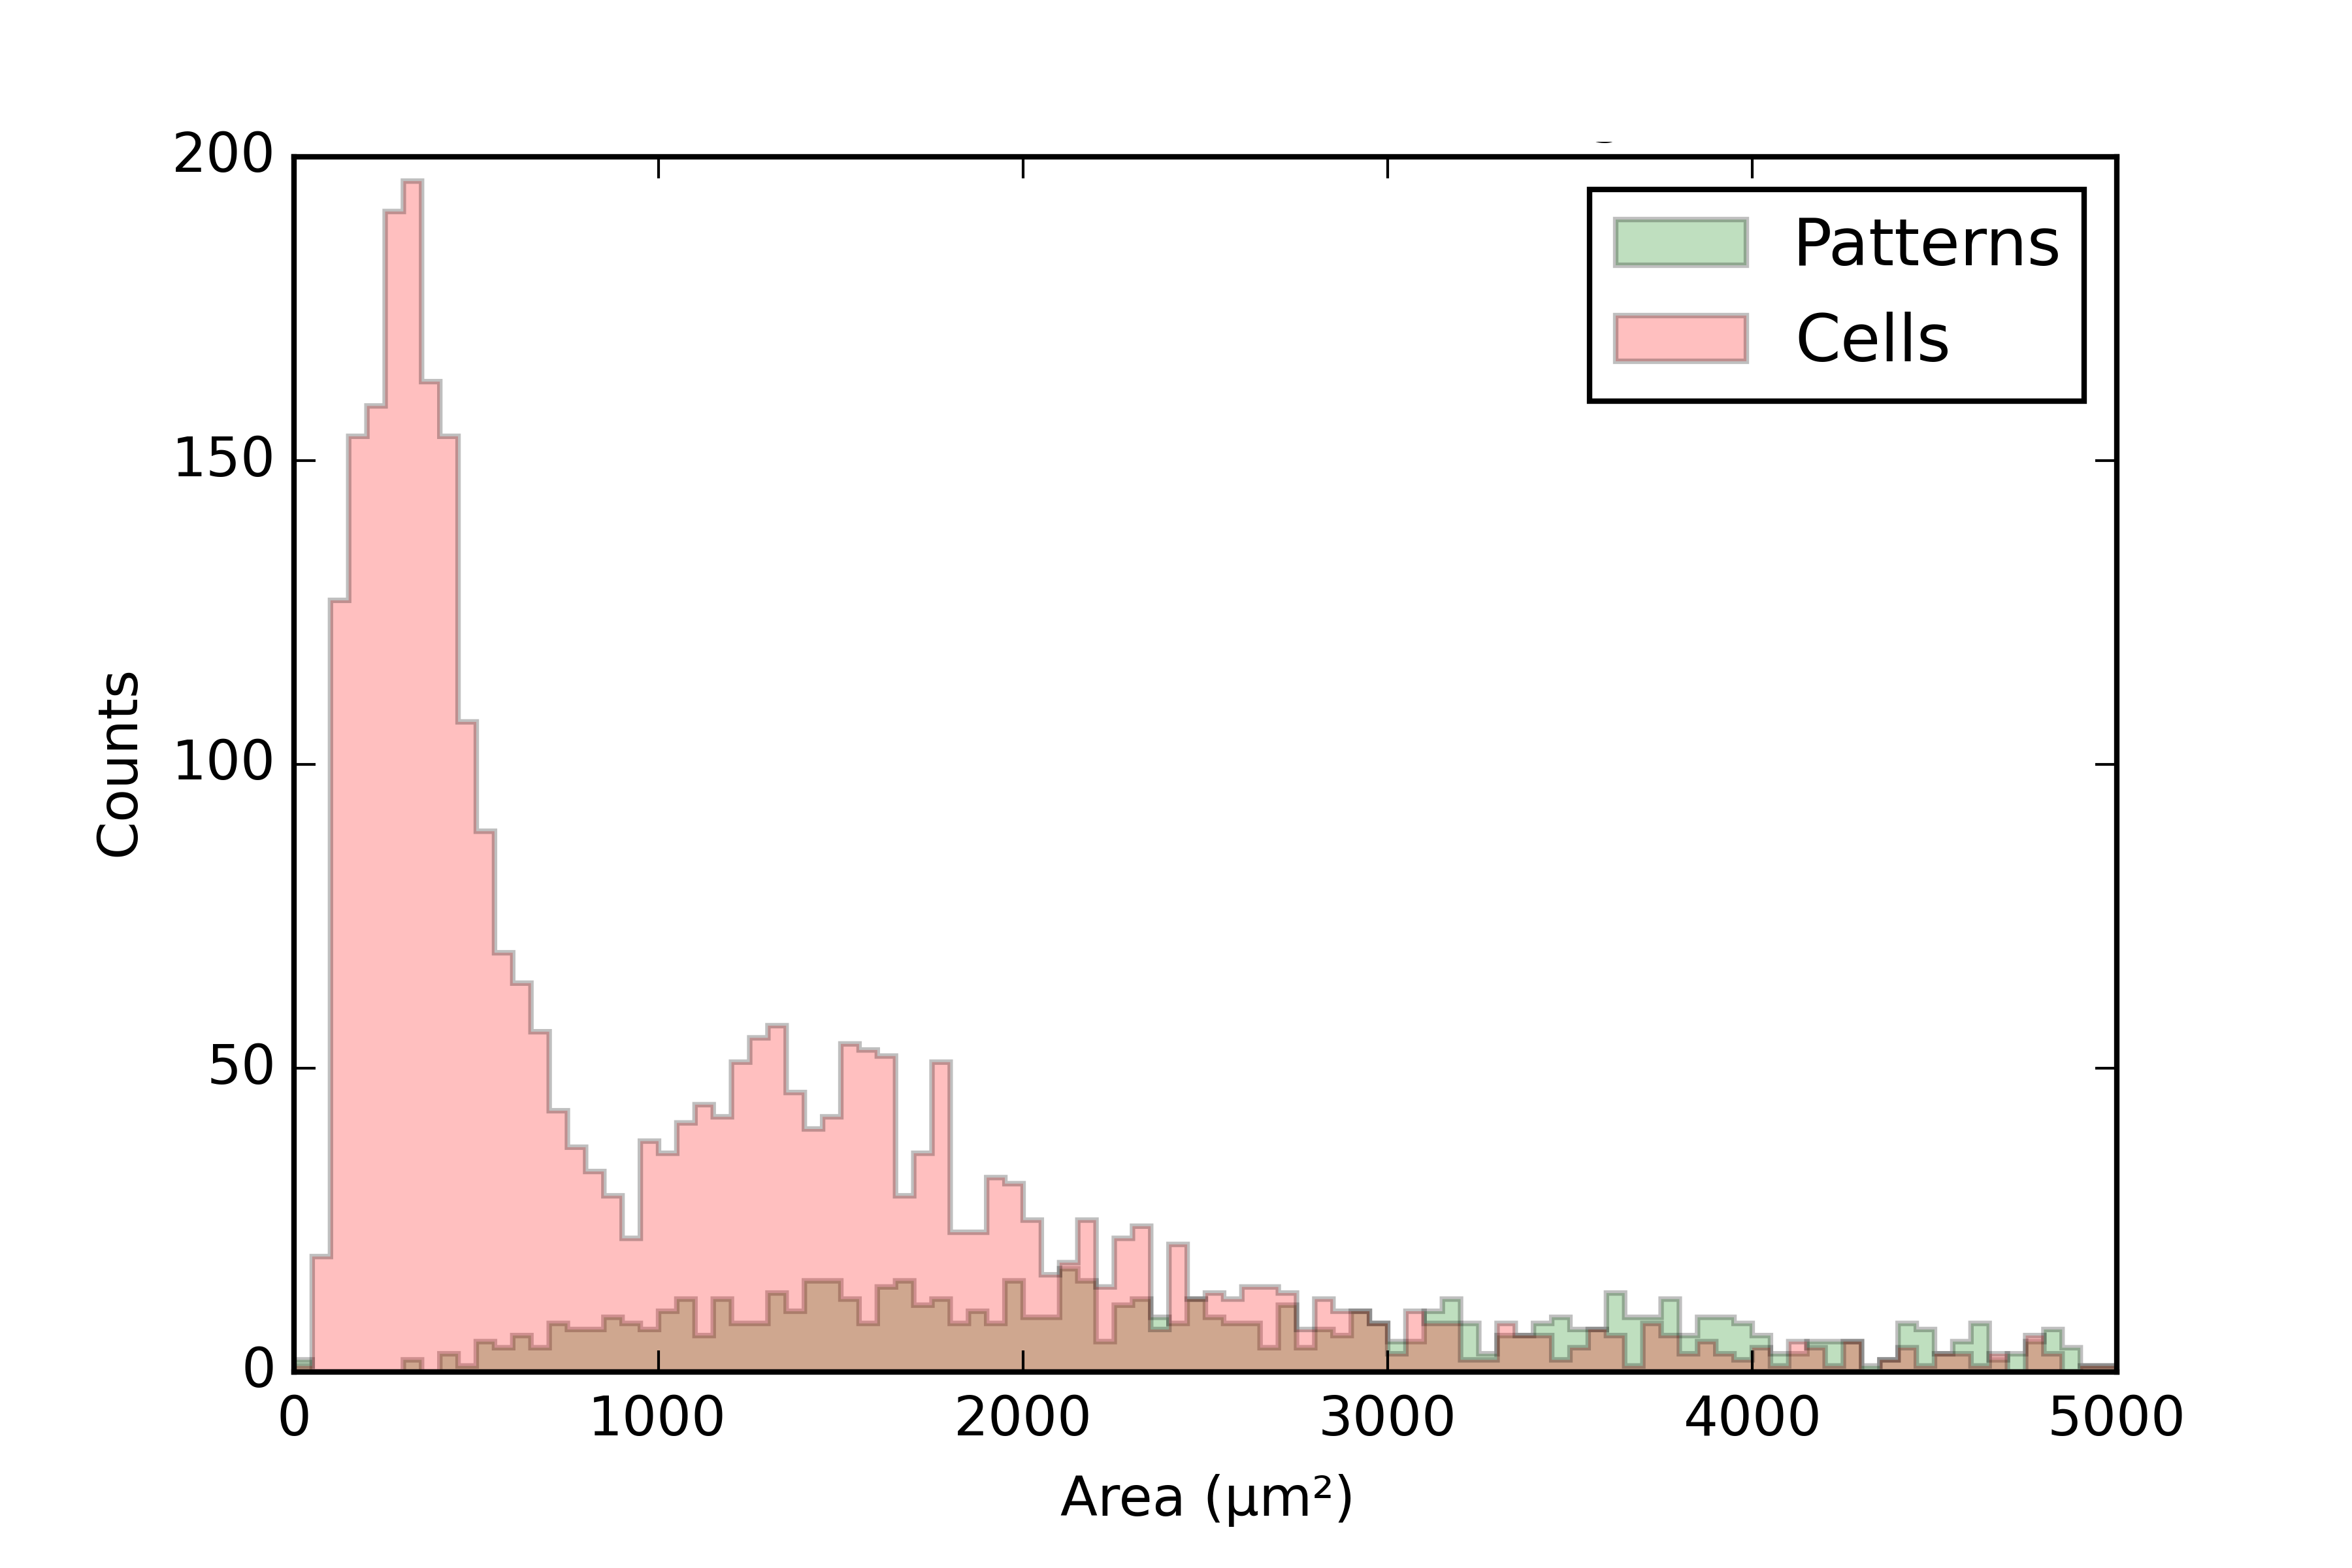
\includegraphics[scale=0.75]{image/cells_patterns_real_area_0_5000.png}
	\caption{Area distributions of the experts' annotations.}
	\label{fig:hist_area_cell_vs_pattern}
\end{figure}

\begin{figure}
	\center
 	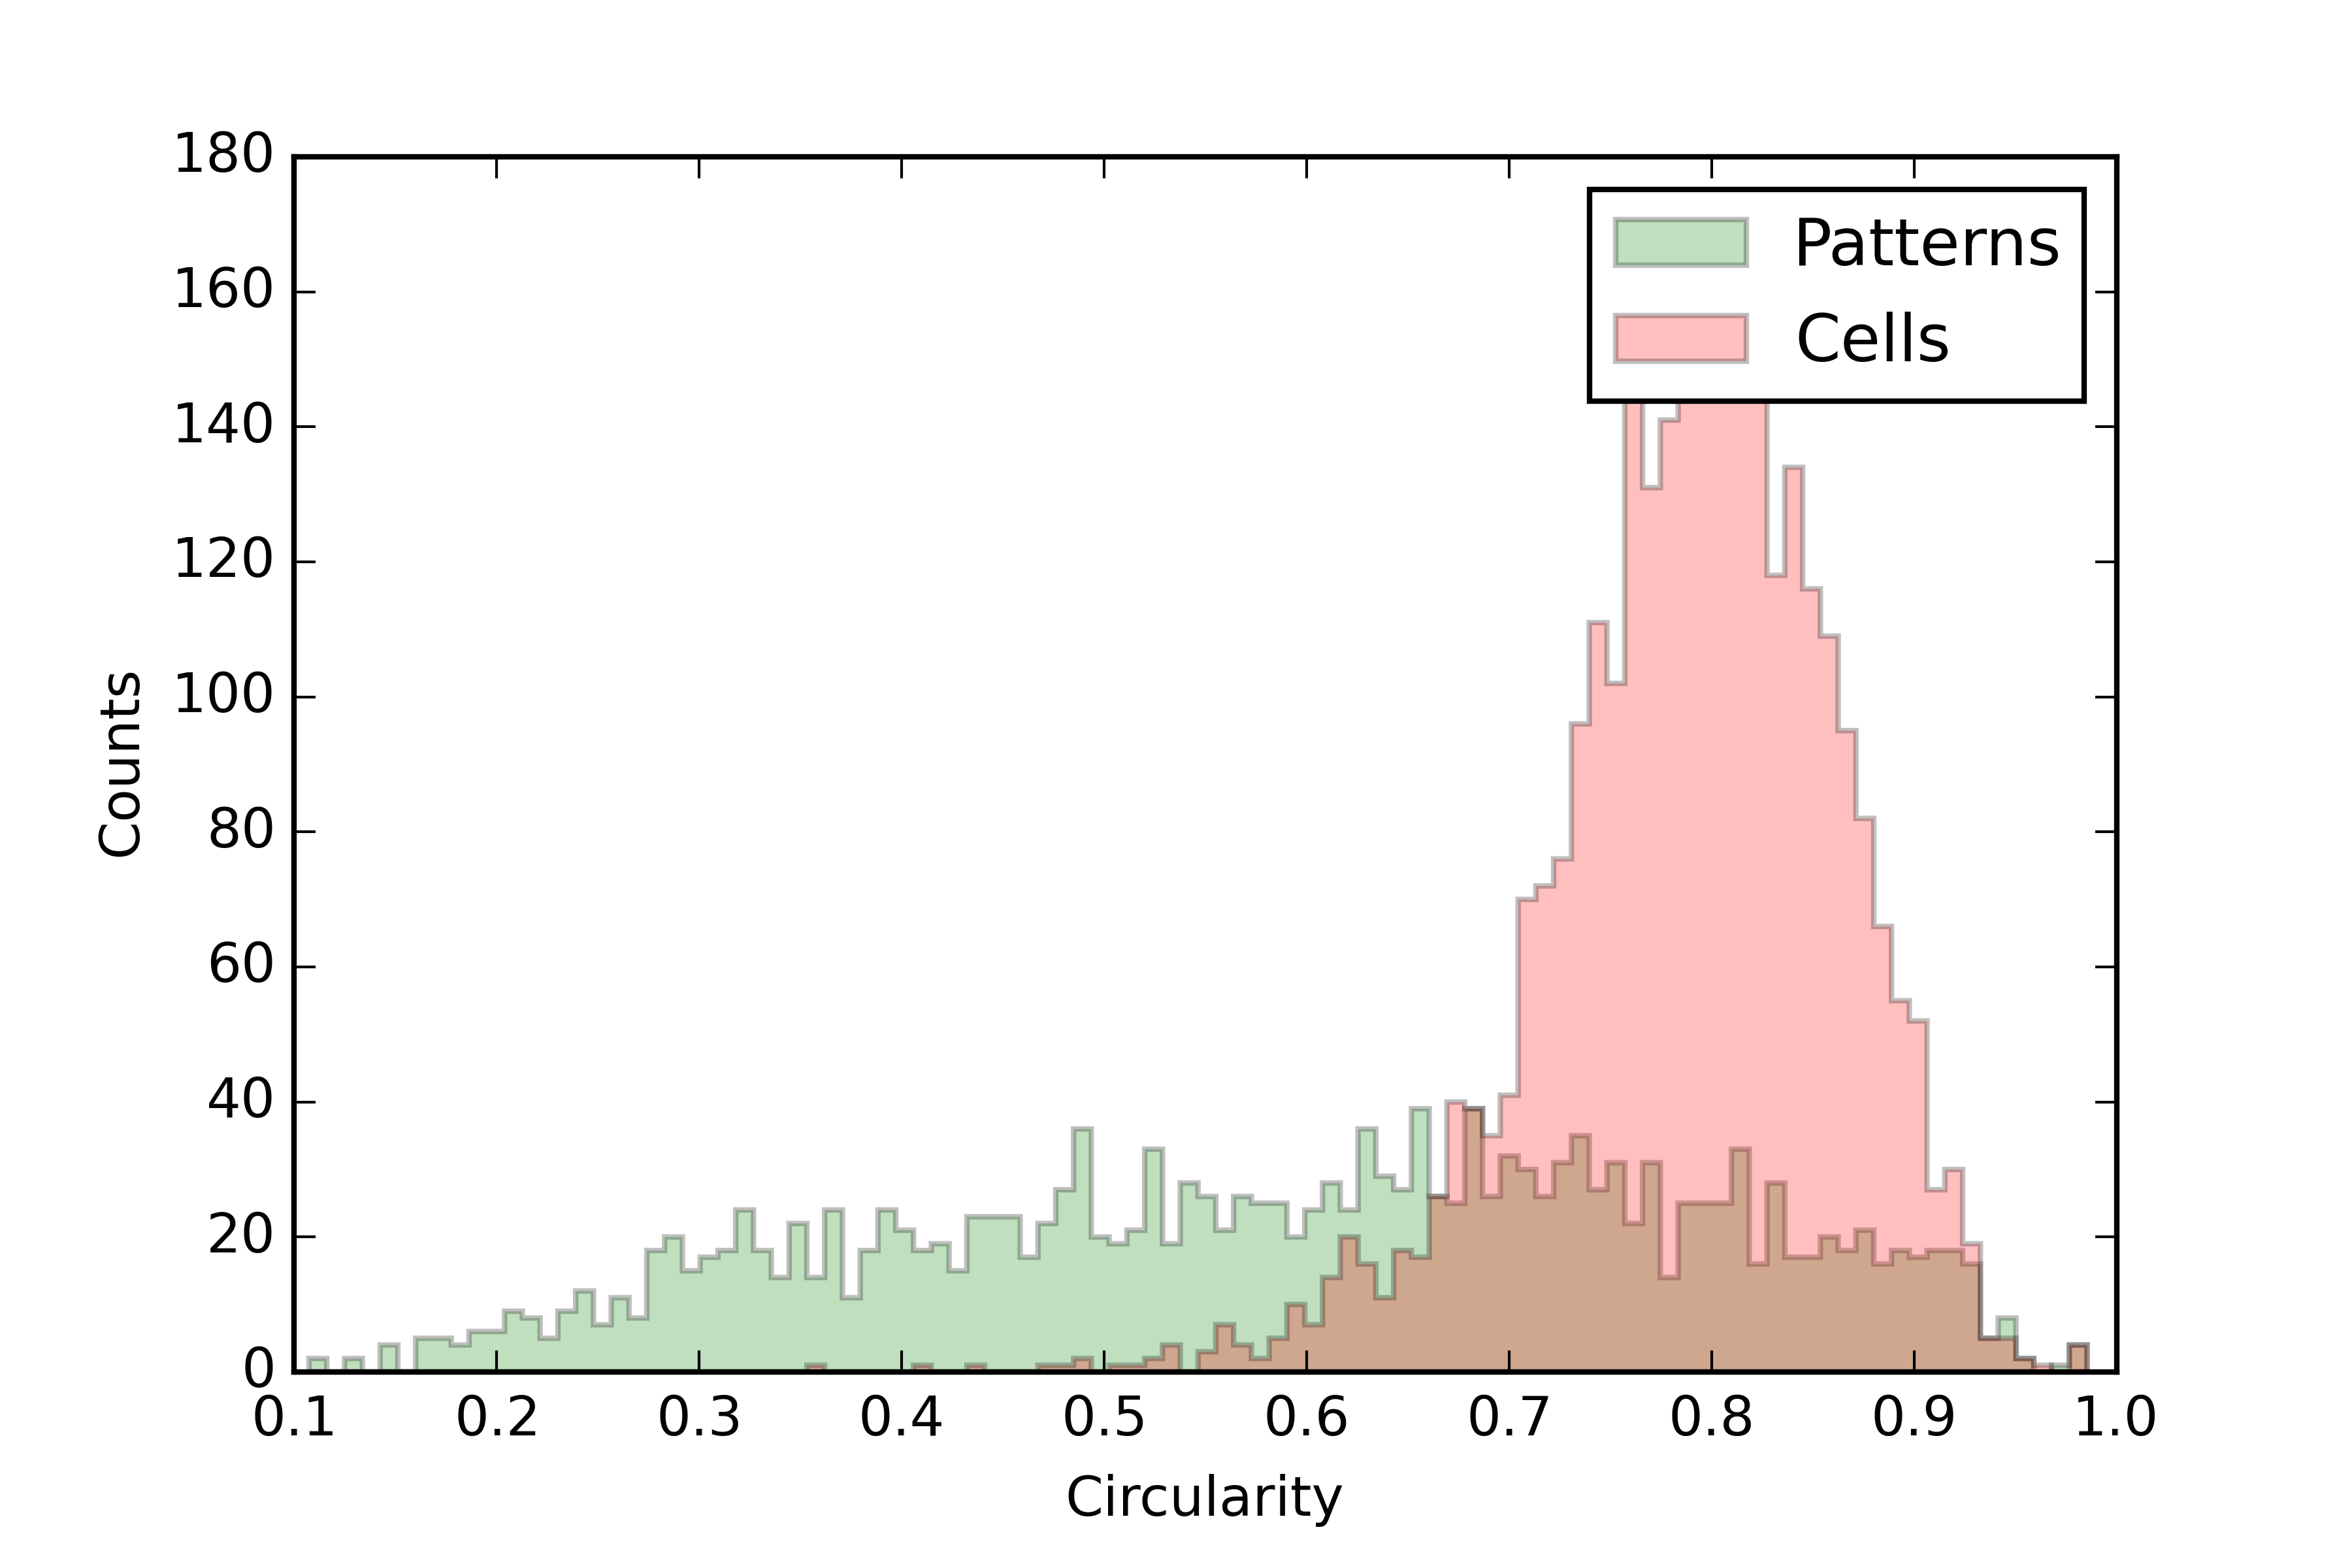
\includegraphics[scale=0.75]{image/cells_patterns_circ.png}
	\caption{Circularity distribution of the experts' annotations.}
	\label{fig:hist_circ_cell_vs_pattern}
\end{figure}


\subsubsection{Improvement}

As relying solely on geometrical properties is not a viable solution, an alternative consists in using the objects' crop image. Especially, the objects' crop would be classified into one of the dispatching categories (i.e. cell, pattern or other) using the random subwindows image classification algorithm \cite{Maree201617} (this algorithm is detailed in Appendix \ref{app:random_subwindows}). A drawback of this solution is that the dimensions of the objects are completely ignored. Given that some patterns might have a similar appearance then cells (color and shape), this might lead to misclassification. 

The overcome the possible problems with the first solution, one could include the geometrical information of the polygons into the learning and prediction processes of the random subwindows algorithm. Especially, the circularity and area would be appended to the feature vector used by the SVM classifier to perform the image classification. This simple operation might not be sufficient however. Indeed, as the features extracted from the ensemble of randomized trees are numerous, the two geometric features would probably not contribute much to the prediction. To overcome this issue, a kernel could be used to increase the contribution of the geometric features. Whereas this solution might yield better results than the first, it requires the experts' annotations of the learning set to be cleaned to avoid the problem mentioned in Section \ref{sec:thyroid_impl_issue}. Moreover, it would require a non-negligible modification of the random subwindows algorithm. It was therefore considered out of the scope of this thesis and the first proposed solution was retained.

\begin{figure}
	\center
	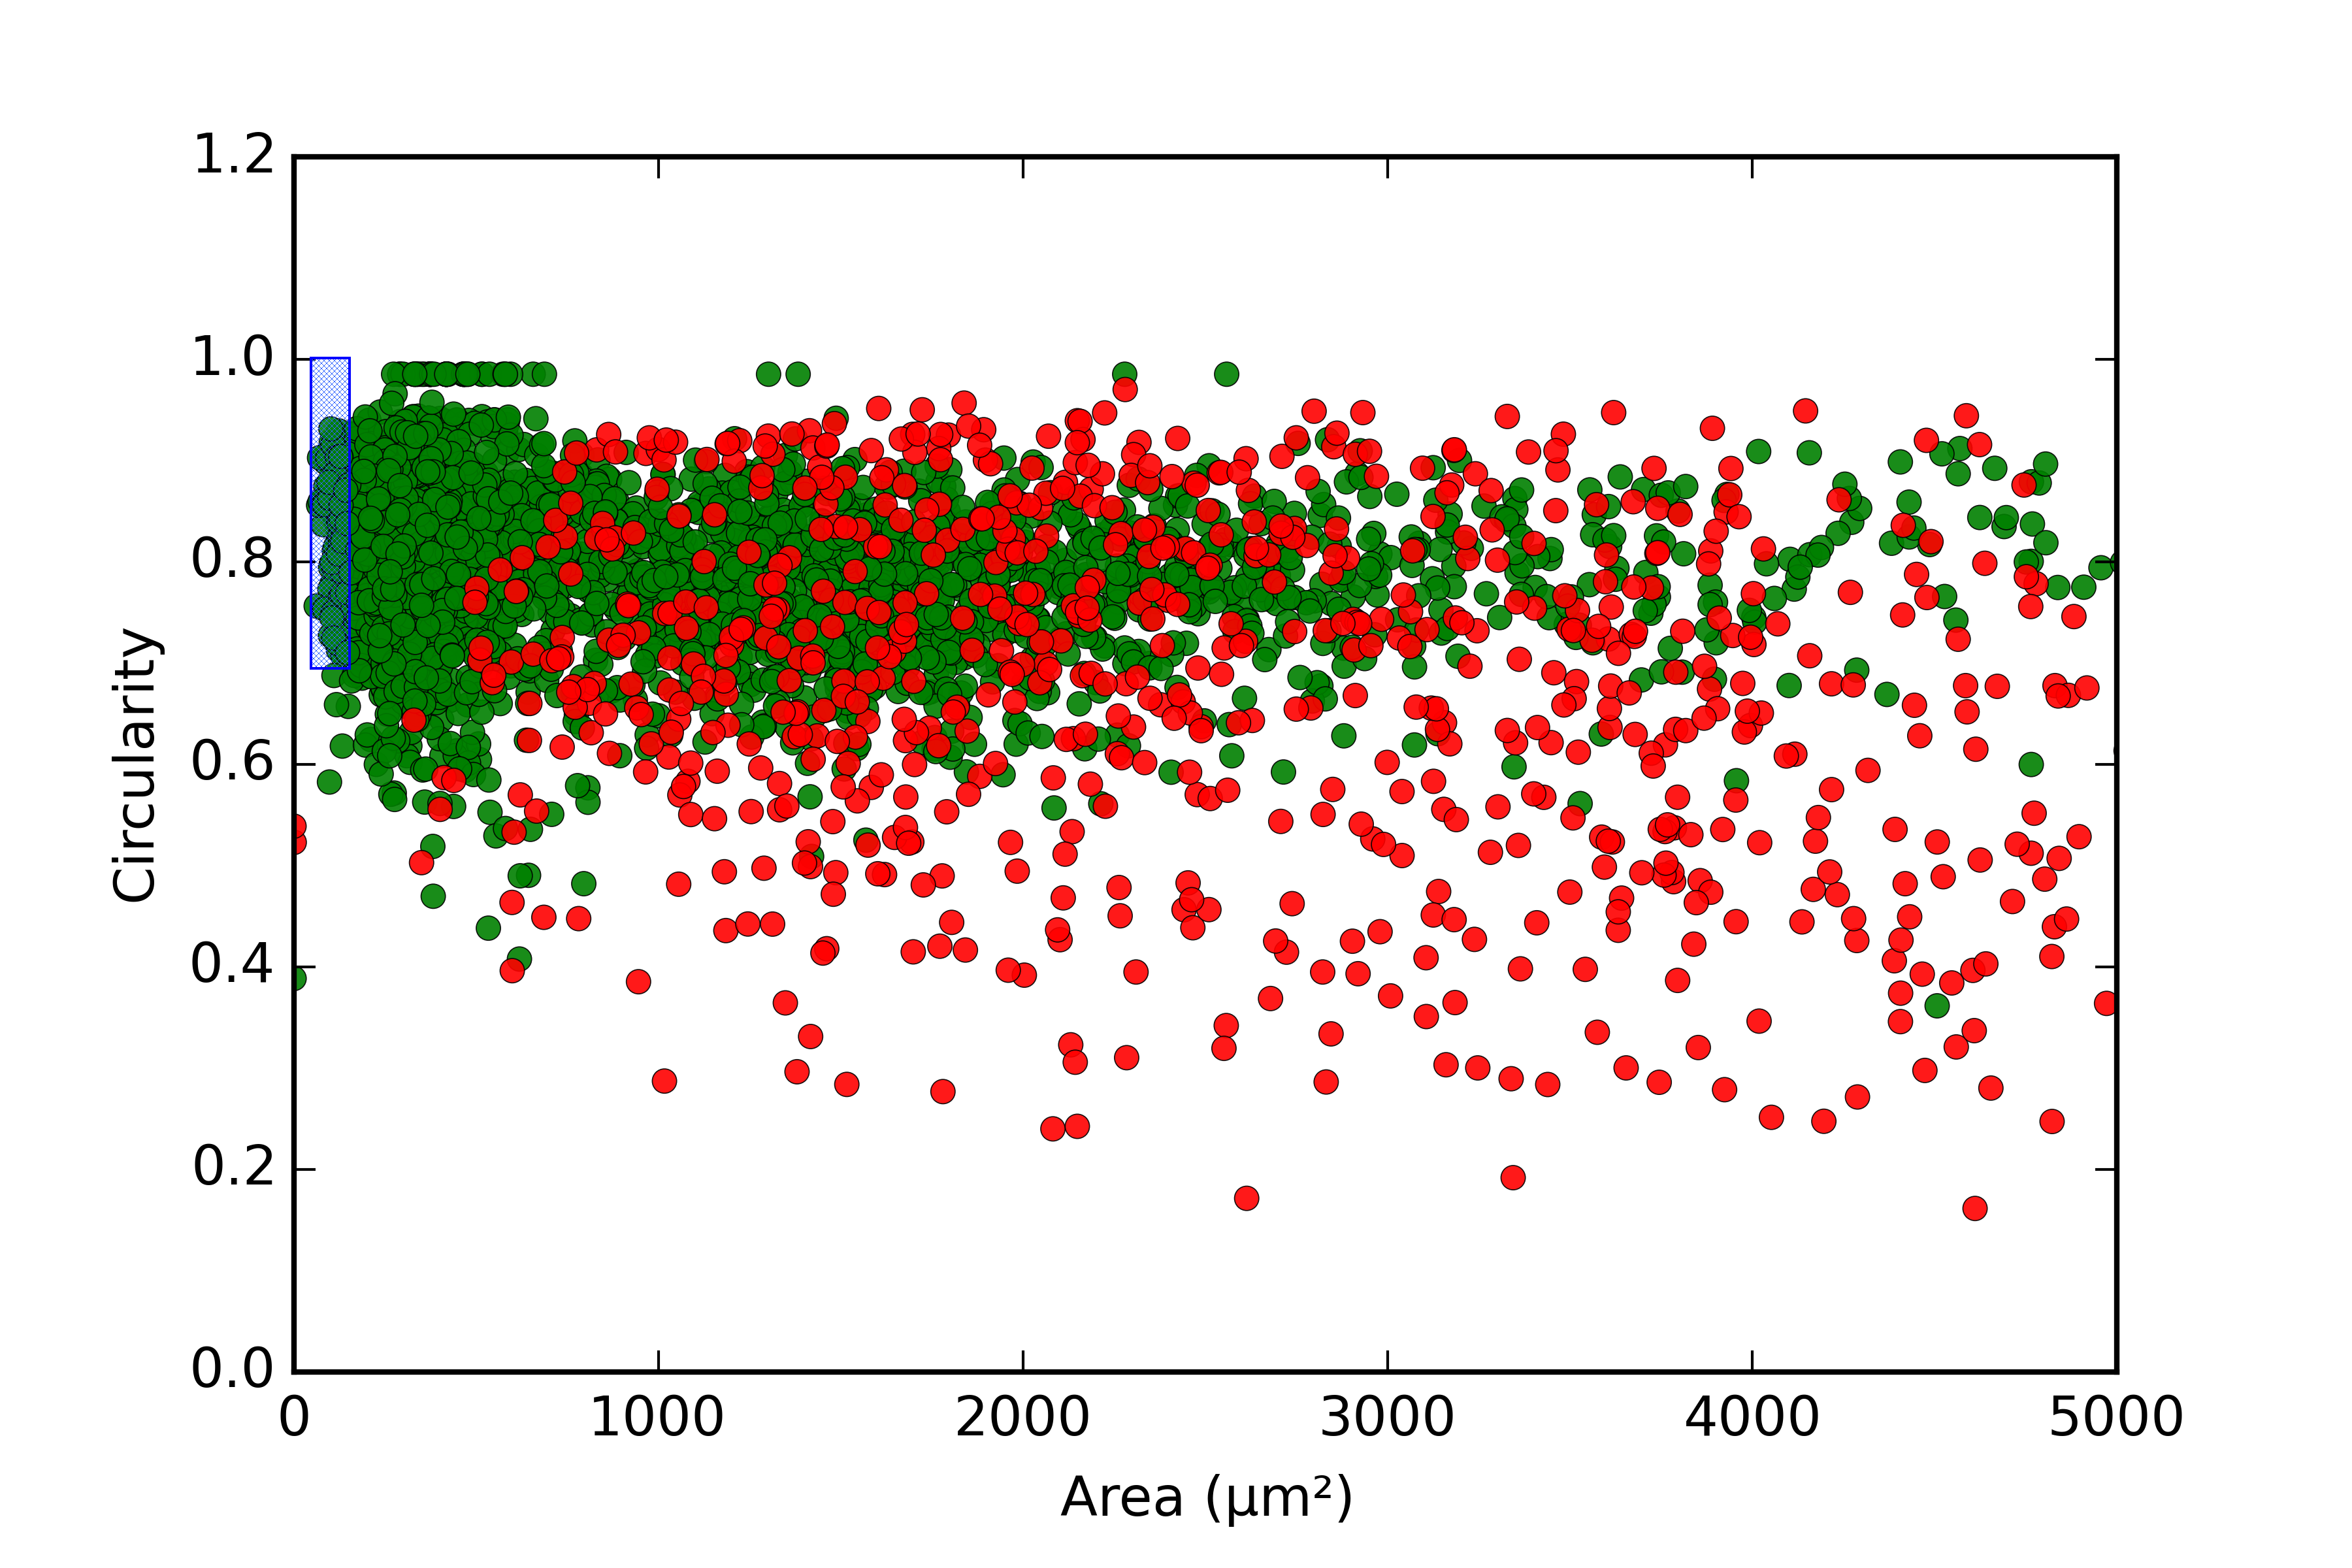
\includegraphics[scale=0.75]{image/scatter_cells_patterns_0_5000.png}
	\caption{Scatter plot, circularity versus area. Green and red dots correspond respectively to cells and patterns. The blue box is the cell dispatching zone.}
	\label{fig:scatter_area_circ_cell_vs_pattern}
\end{figure}

\subsection{Classification}

As soon as objects are dispatched, they have to be classified. In \cite{adeblire2013}, the author uses two classification models: one for cells and another one for patterns. For patterns, a ternary classifier is used and predicts three classes: \textit{proliferative pattern}, \textit{non-proliferative pattern} and \textit{others}. The author states that the third class is needed because with a binary classifier, some objects were classifieed as patterns while they were not. Hopefully, with the new dispatching procedure, those objects will be eliminated before reaching the classifier. It was therefore decided to use a binary classifier for performing this classification. 

As far as the cell classifier is concerned, it predicts two classes: \textit{cells with inclusion} and \textit{non-inclusion}. In addition to the term \textit{cell with inclusion}, the author includes the pseudo inclusions in the positive class. 

The performance study for the various classifiers is given in Section \ref{ssec:thyroid_perf_models}.

\section{Implementation}
\label{sec:thyroid_implementation}
Following the \textit{SLDC} framework philosophy, the problem dependent components have to be defined: an image representation, the segmentation procedures, the dispatching rules and the classifiers. Whenever possible, the components were developed to be reusable for other applications within Cytomine. Those generic components are colored in blue in UML diagrams while the components dependent on the thyroid problem are colored in green.

\subsection{Image representation}

\begin{figure}
	\center
	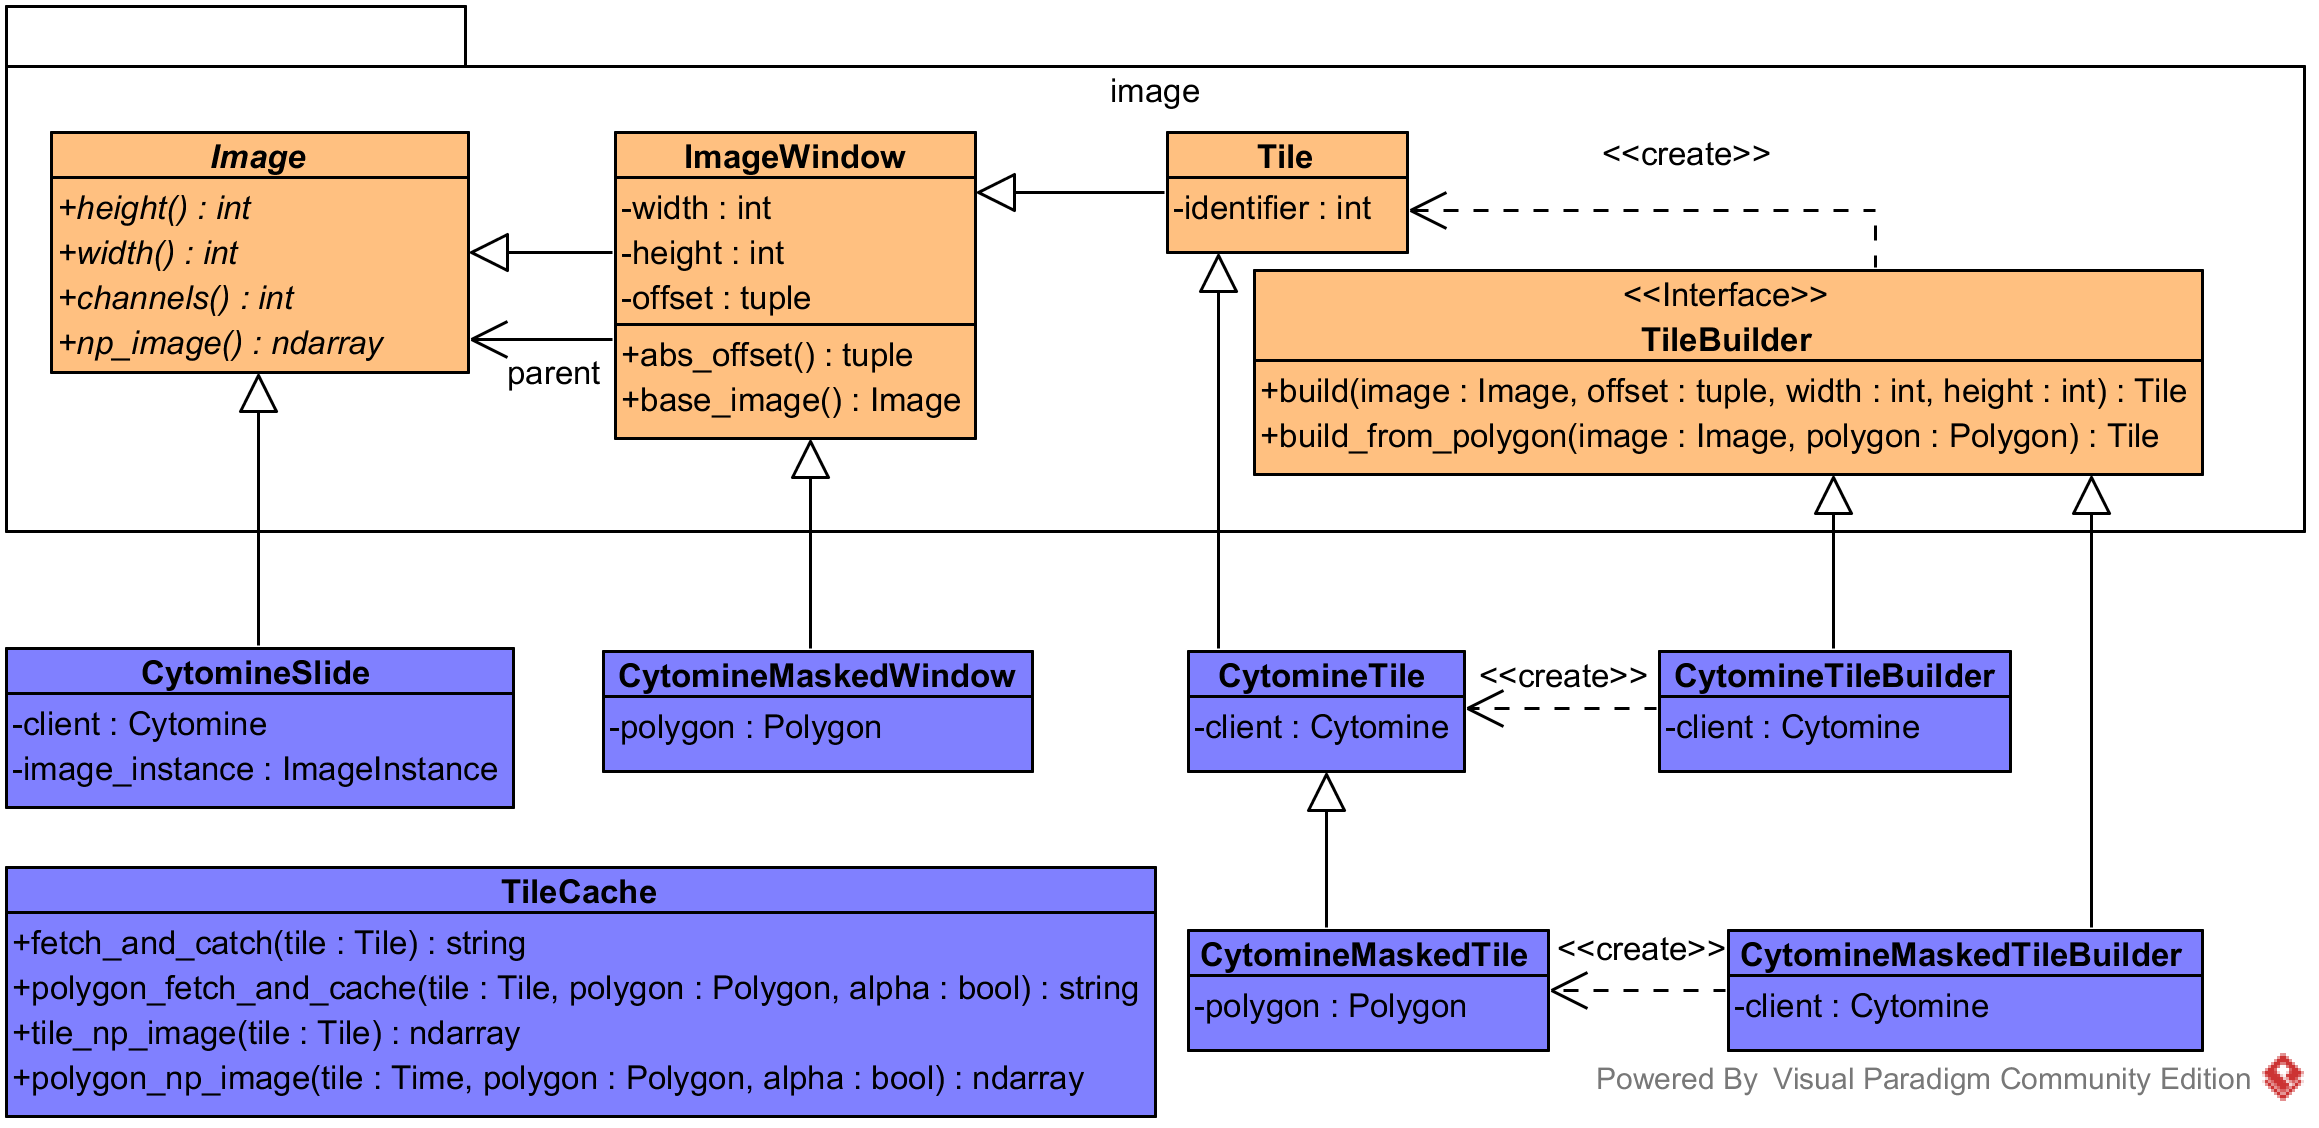
\includegraphics[scale=0.85]{image/thyroid_image.png}
	\caption{UML diagram - Cytomine image representation}
	\label{fig:uml_cyto_im_repr}
\end{figure}

\subsection{Dispatching rules}

\begin{figure}
	\center
	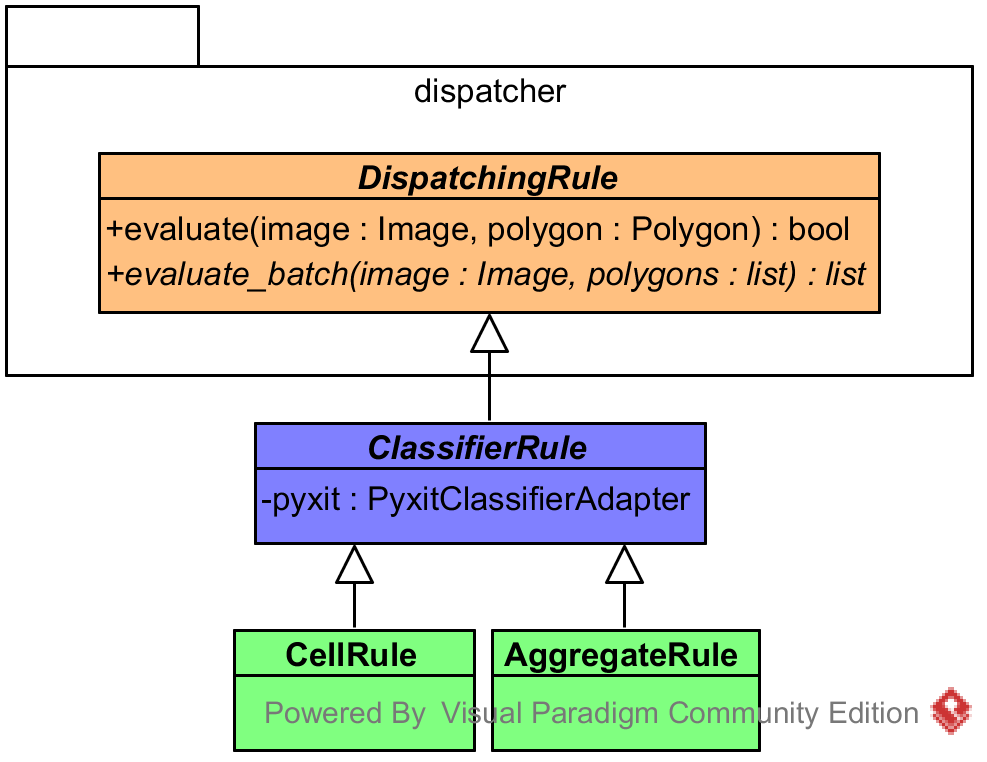
\includegraphics[scale=0.85]{image/thyroid_dispatching_rules.png}
	\caption{UML diagram - Thyroid workflow dispatching rules}
	\label{fig:uml_cyto_disp_rules}
\end{figure}

\subsection{Segmentation}

\begin{figure}
	\center
	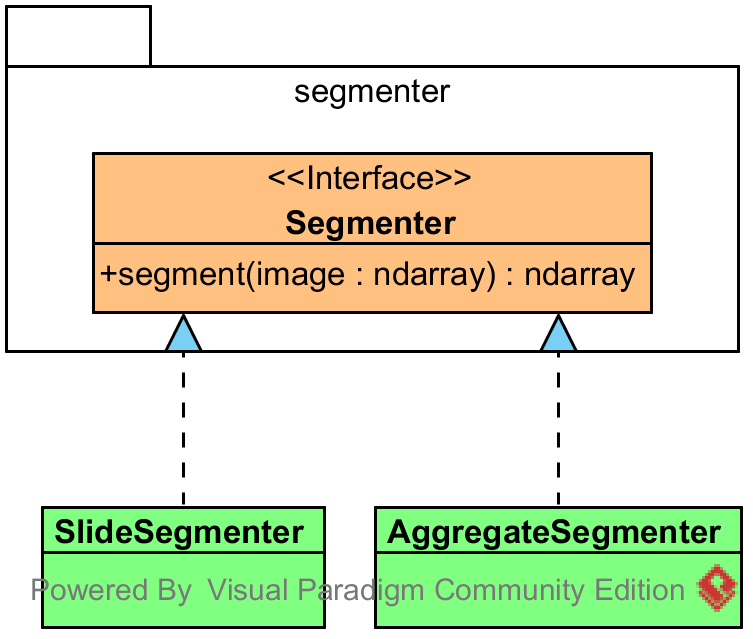
\includegraphics[scale=0.85]{image/thyroid_segmenters.png}
	\caption{UML diagram - Segmenter classes}
	\label{fig:uml_cyto_segmenters}
\end{figure}

\subsection{Classifier}

\begin{figure}
	\center
	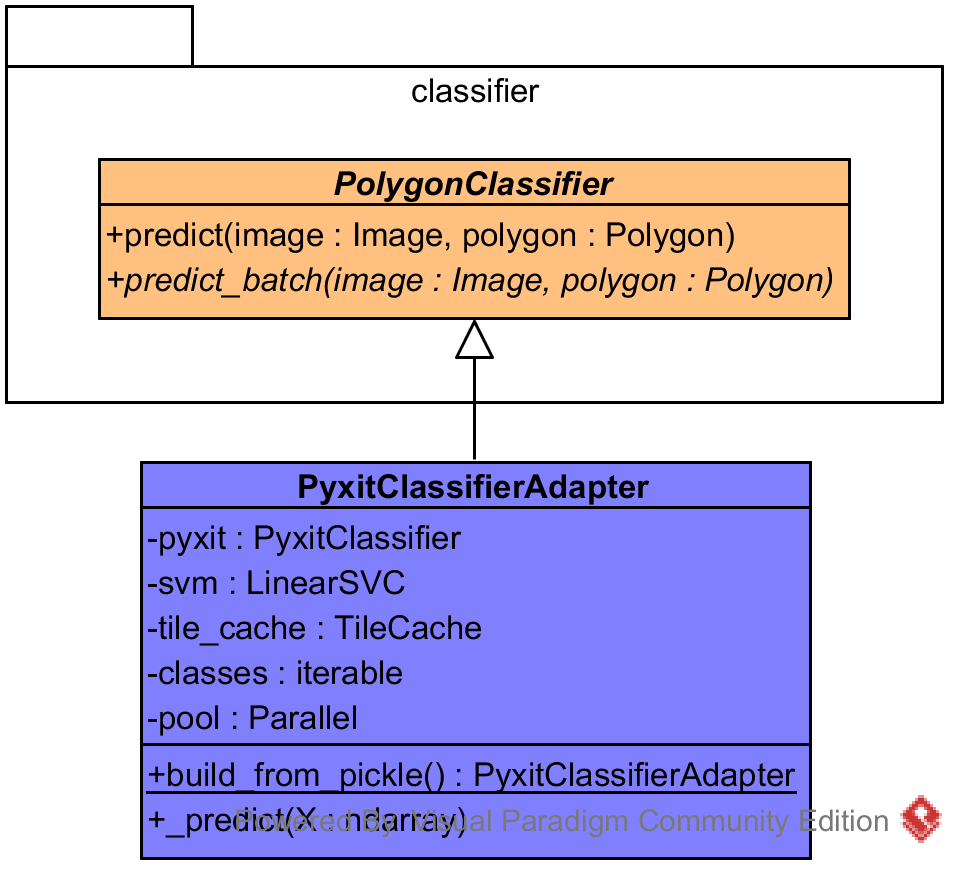
\includegraphics[scale=0.85]{image/thyroid_classifiers.png}
	\caption{UML diagram - Classifier}
	\label{fig:uml_cyto_classifiers}
\end{figure}

\subsection{Chaining}

\begin{figure}
	\center
	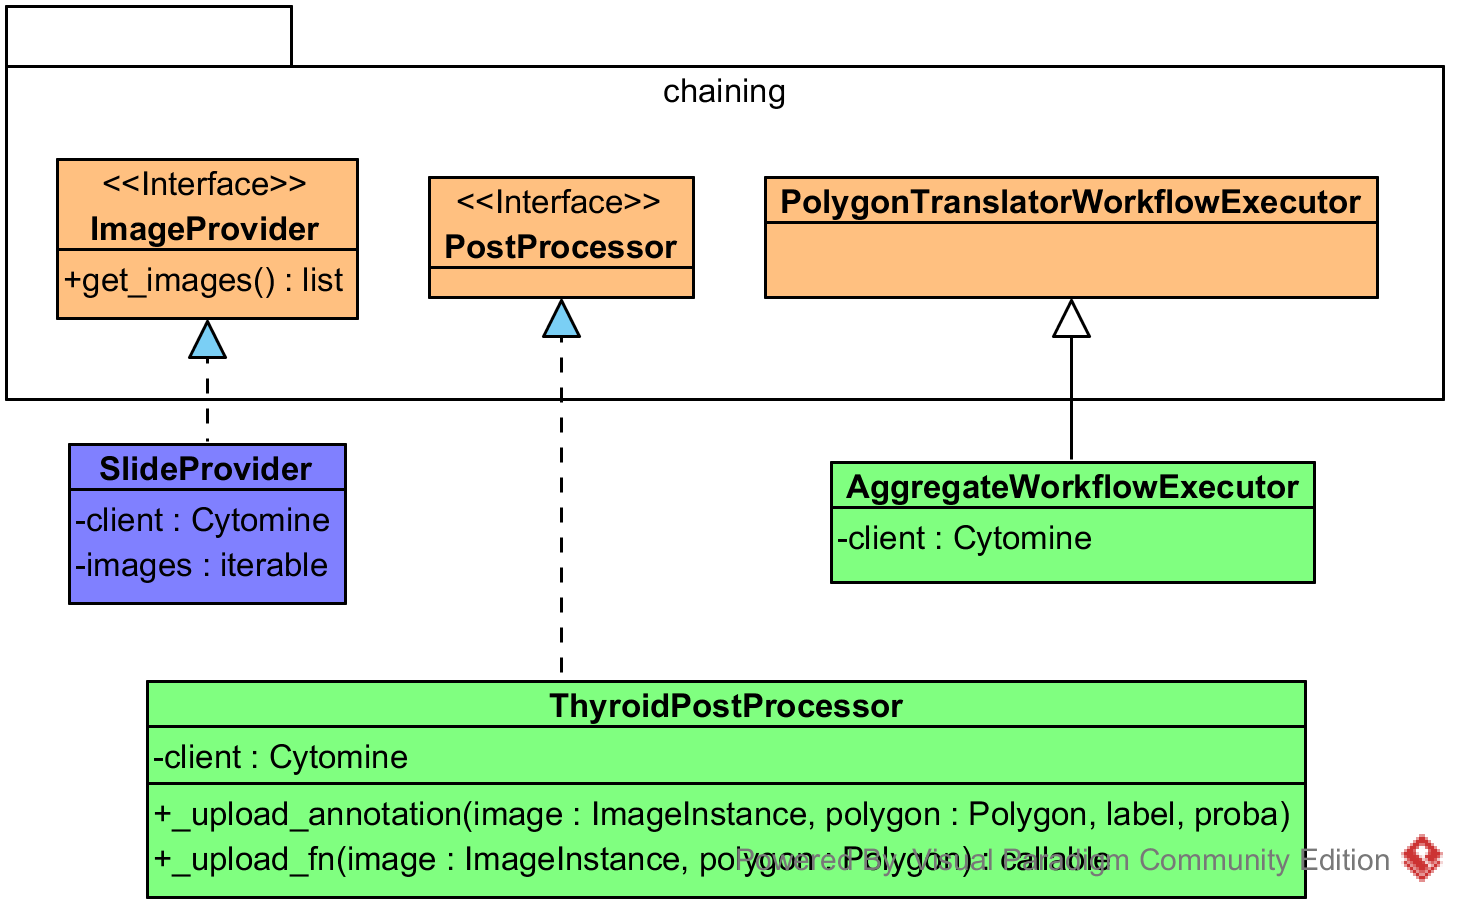
\includegraphics[scale=0.85]{image/thyroid_image_provider.png}
	\caption{UML diagram - Chaining classes}
	\label{fig:uml_cyto_chaining}
\end{figure}


\section{Performance analysis}
\label{sec:thyroid_perf}

\subsection{Classification models}
\label{ssec:thyroid_perf_models}
\subsubsection{Test set and cross validation}
\subsubsection{Dispatching model}
\subsubsection{Pattern classifier}
\subsubsection{Cell classifier}

\subsection{Execution times}

\subsection{Memory}

\subsection{Overall}